
\chapter{Results and Discussion for ACL and HOL Verification}
\label{cha:results-disc-acl}

\section{File and Folder Structure}
\label{sec:file-fold-struct}

\subsection{ABD Folder}
\label{sec:abd-folder-1}


The overall layout of the ABD folder was shown in figure 5.1.  The Documentation folder contained
the documentation.  The PatrolBase folder contained the original secure state machine diagrams
and other translations of the patrol base operations into verifiable formats.  The HOL folder
contained all the HOL codes and EmitTeX reports. 
  \begin{figure}[h]
  \centering
  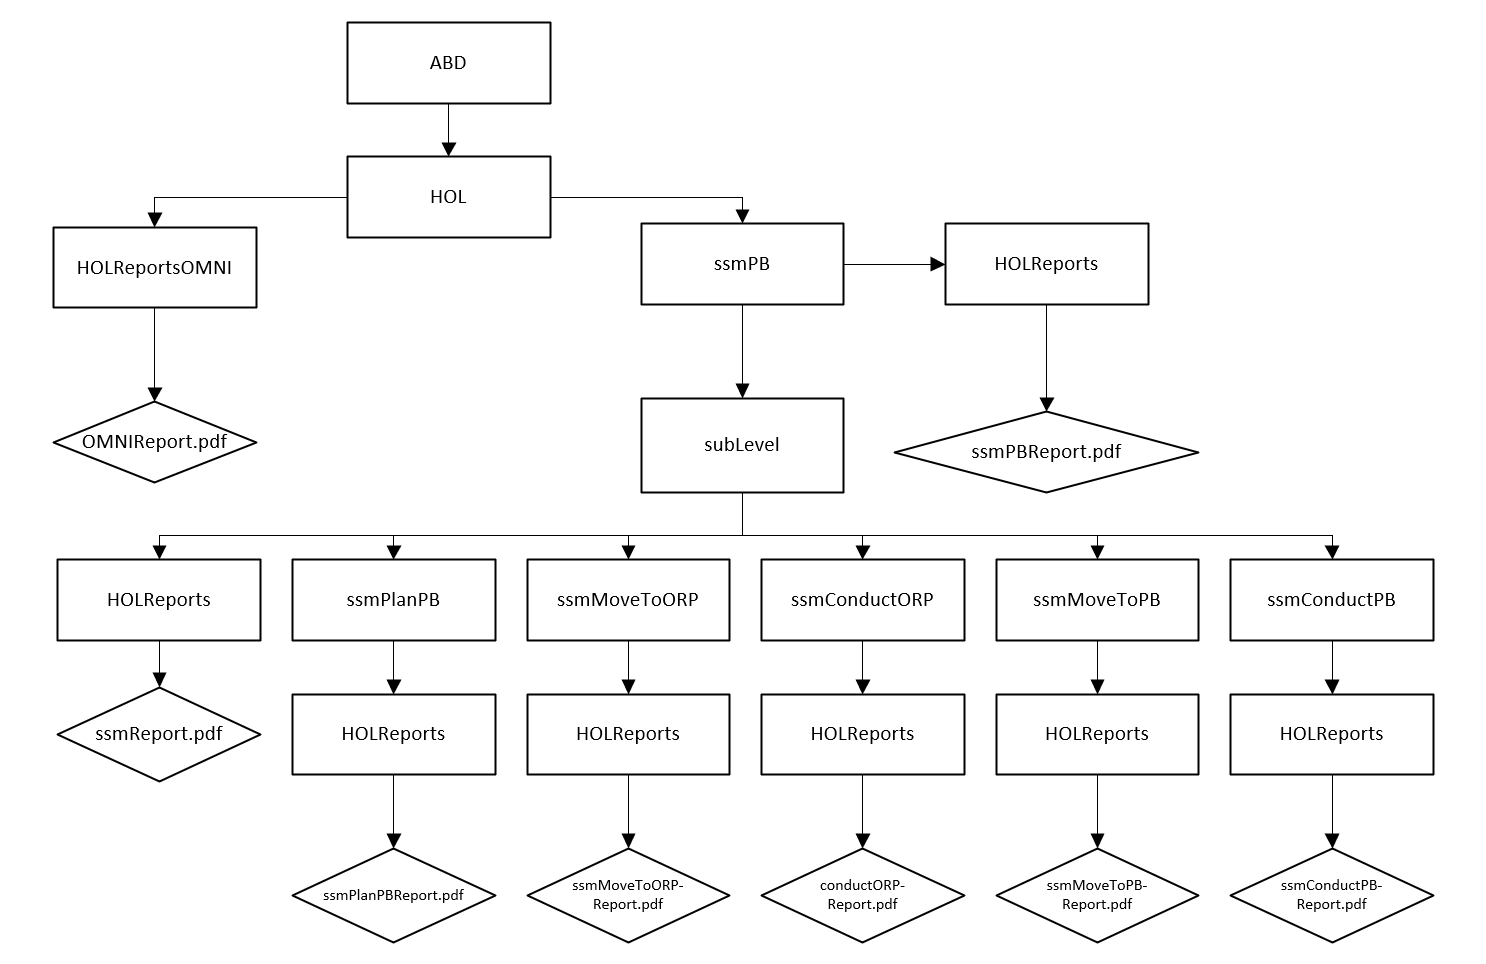
\includegraphics[width=0.9\linewidth]{ABDfolder.PNG}
  \caption{ABD Folder Structure}
\end{figure}

\subsection{Documentation Folder}
\label{sec:documentation-folder-1}


\subsection{PatrolBase Folder}
\label{sec:patrolbase-folder-1}


\subsection{HOL Folder}
\label{sec:hol-folder-1}


Figure 5.2 showed the OMNI-level folder.  OMNI-level contained files and folders that were
used by the entire HOL portion of the project. 
\begin{figure}[h]
  \centering
  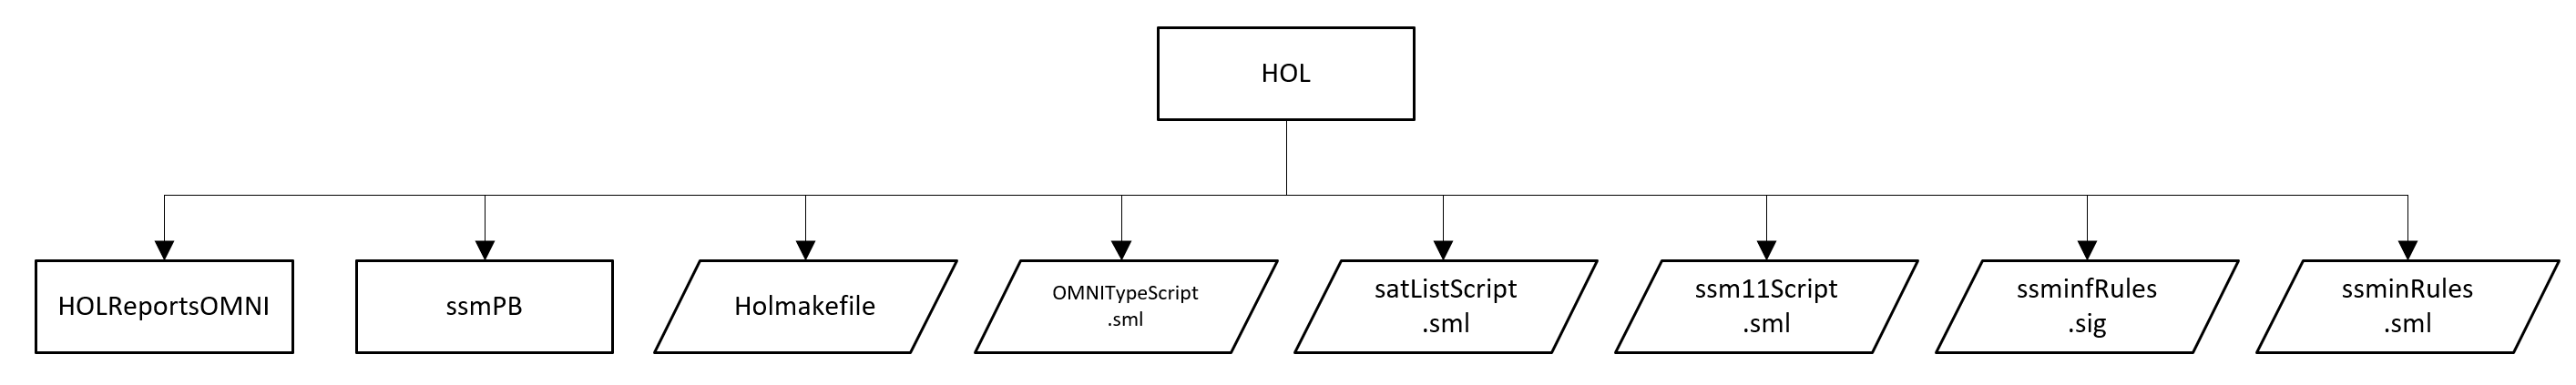
\includegraphics[width=1\linewidth]{HOLOMNI.PNG}
  \caption{HOL OMNI-level Folder}
\end{figure}\\

\subsubsection{HOLReportsOMNI}
\label{sec:holreportsomni-1}


HOLReportsOMNI contained the code necessary to generate the pretty-printed EmitTeX
documentation for all theories in the project.  EmitTeX converted ALL the datatypes
and theorems in the *.Script.sml files into pretty-printed text and saved it in
OMNIReport.pdf.  A copy of OMNIReport.pdf was included in the appendix.  HOLReportsOMNI
contained the same kinds of files as all HOLReports folders, which was described below.  


\subsubsection{ssmPB}
\label{sec:ssmpb-1}


Figure 5.3 showed the files and folders in ssmPB.  ssmPB was the top-level secure
state machine.  It contained two theories: PBTypeScript.sml and ssmPBScript.sml.
PBTypeScript.sml contained the type definitions for the top-level secure state machine
defined in ssmPBScript.sml.  The subLevel folder contained the sub-level secure state machines.

\begin{figure}[h]
  \centering
  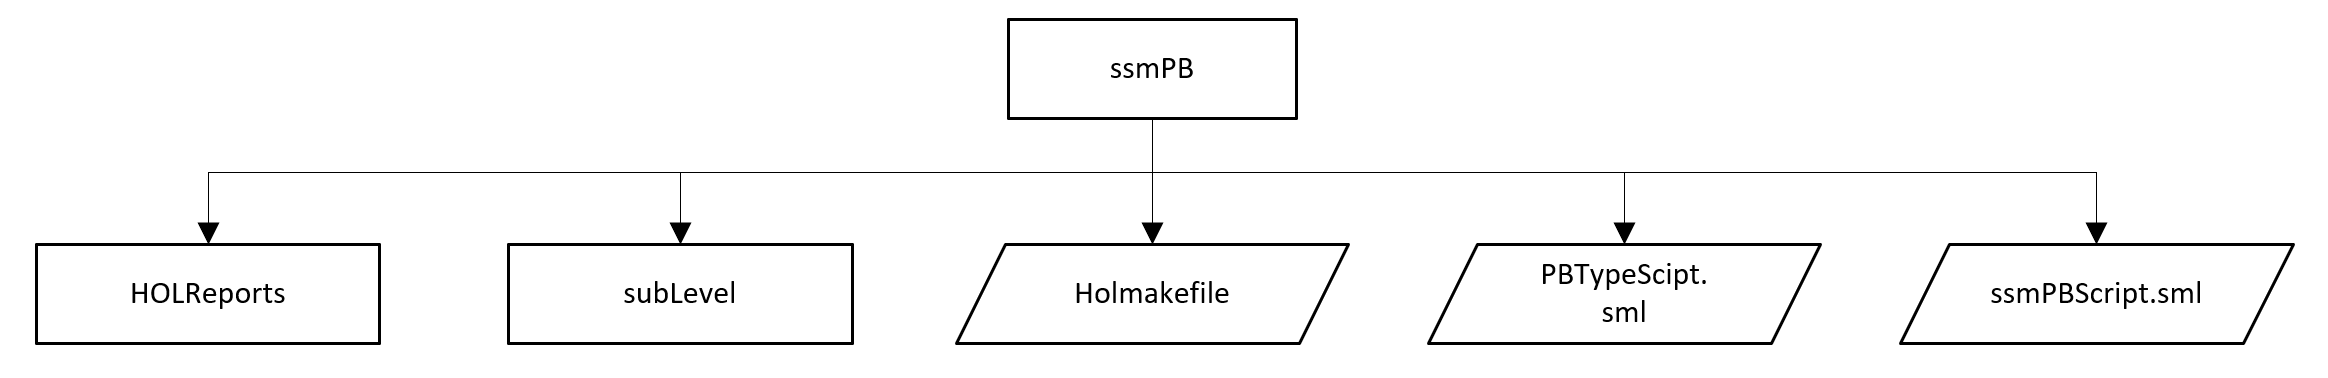
\includegraphics[width=1\linewidth]{ssmPB.PNG}
  \caption{ssmPB, Example of a Secure State Machine Folder}
\end{figure}

\underline{subLevel}


The subLevel folder contained the folders for the sub-level secure state machines.
The contents were similar to ssmPB.  Each folder contained two script files,
one defining the secure state machine datatypes and the other containing the
secure state machine definition.


\subsubsection{OMNITypeScript.sml}
\label{sec:omnitypescript.sml-1}


OMNITypeScript.sml contained definitions for datatypes used in all secure state machines.


\subsubsection{satListScript.sml, ssminfRules.sig and ssminfRules.sml}
\label{sec:satl-ssminfr-ssminfr-1}



satListScript.sml, ssminfRules.sig and ssminfRules.sml contained theories that the
parameterizable ssm11 and ssm needed to work properly.


\subsection{HOLReports}
\label{sec:holreports-1}


Figure 5.4 showed the contents of a typical HOLReports folder.  Each HOLReports folder,
except for HOLReportsOMNI, contained the files necessary to generate the pretty-printed
EmitTeX documentation for the theories in the immediate super folder.  The HOLReportsOMNI
folder contained the files necessary to generate the pretty-printed documentation for
ALL the theories in the project.  EmitTeX converted the datatypes, definitions, and
theorems in the *Script.sml files into pretty-printed text and saved the results in *Report.pdf.
For HOLReportsOMNI, the documentation was saved in OMNIReport.pdf.  A copy of OMNIReport.pdf
was included in the \textbf{appendix?}.  

\begin{figure}[h]
  \centering
  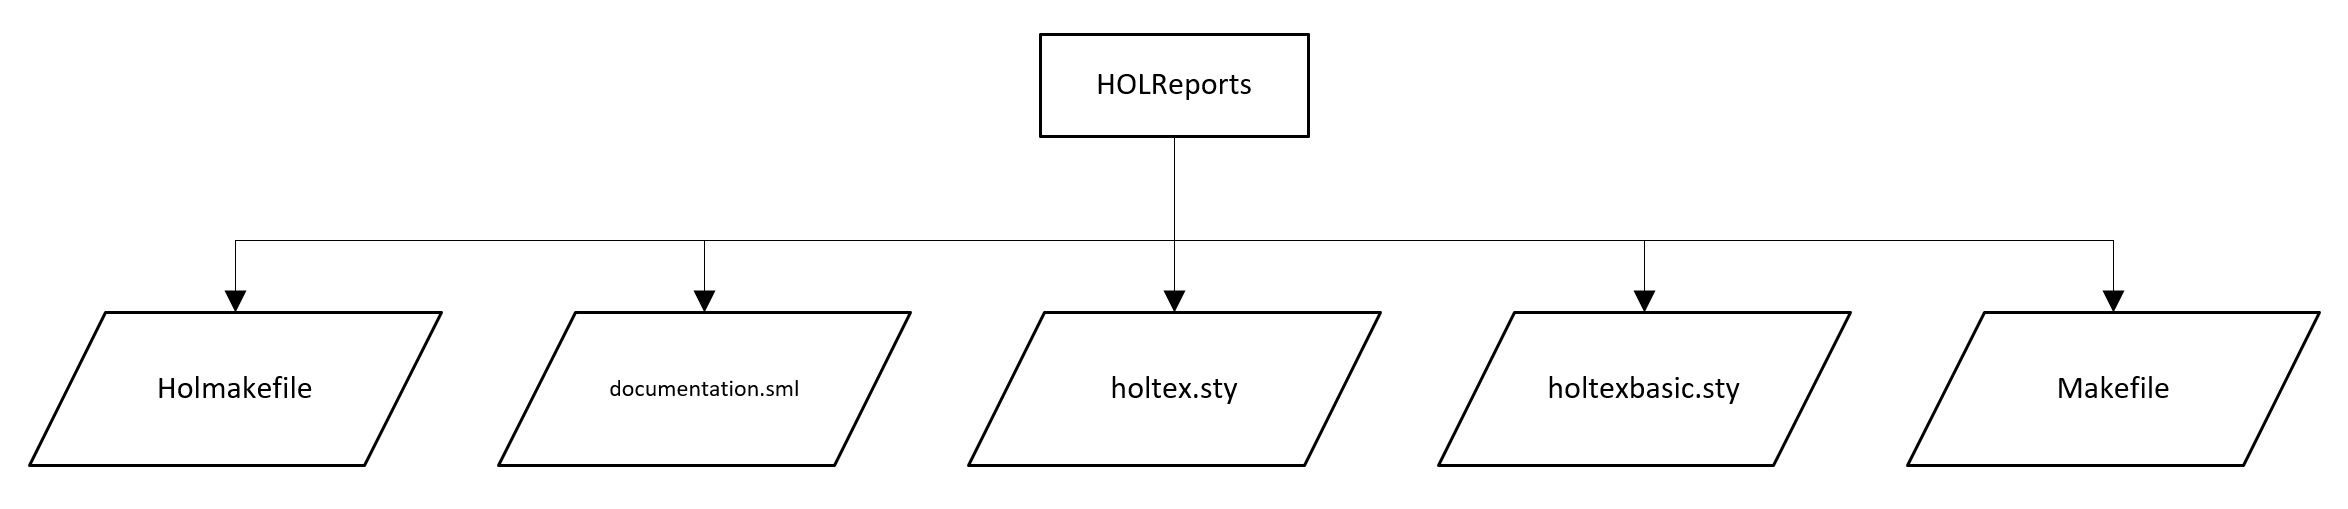
\includegraphics[width=1\linewidth]{HOLreport.PNG}
  \caption{HOLReports}
\end{figure}


\subsubsection{Documentation.sml}
\label{sec:documentation.sml-1}


documentation.sml loaded EmitTeX and the required *Script.sml files into HOL.
It then opened EmitTeX and applied the print_theories_as_tex_doc function on the *Script.sml files.

\subsubsection{holtex.sty and holtexbasic.sty}
\label{sec:holt-holt-1}


holtex.sty and holtexbasic. sty were style files that told HOL how to format the
HOLReport.pdf file generated by EmitTeX.


\subsubsection{Makefile}
\label{sec:makefile-1}



Makefile told the command prompt to send documentation.sml to HOL.  It then
instructed HOL to produce the pdf report using PDFLATEX and MAKEINDEX.



\subsubsection{Holmakefile}
\label{sec:holmakefile-1}


Holmakefile was included in all folders.  This file told Holmake where to
find the theory files necessary to run Holmake.  


\section{State Machines and Secure State Machines: Transition Types and Principals}
\label{sec:state-mach-secure}



What distinguished a state machine from a \textit{secure} state machine was the
  addition of transition states and principals.  The state machine was defined
  by the allowable states and commands (inputs).  The state machine was modified
  to produce a \textit{secure} state machine.  The \textit{secure} state machine imposed restrictions
  on whether or not a state machine could change states.  This implemented the
  principles of complete mediation.  These restrictions were expressed as transition
  types.  The transition types \textit{exec, trap,} and \textit{discard} determined whether a command
  was allowed to be executed, trapped, or discarded, respectively.  Because HOL
  is a strongly-typed language, we also needed one more type called an option type.
  The option type allowed us to return \textit{SOME} command or indicate that there was \textit{NONE}.
  When combined, commands in a \textit{secure} state machine took one of three forms: \textit{exec
  (SOME cmd), trap (SOME cmd),} or \textit{discard (SOME cmd).  exec (SOME cmd)} was executed.
  \textit{trap (SOME cmd)} and \textit{discard (SOME cmd)} were not.  In addition, \textit{trap (SOME cmd)} was
  reduced to \textit{trap NONE} in some of the theorems.  This reduction effectively nullified
  the command \textit{cmd} (because trapped commands were not executed).\\
  
 Trapped commands were not necessary for our project.  Trapped commands
  had a specific function in the virtual machine world for which the original
  parameterizable secure state machine ssm11 was implemented.  In our project,
  trapped commands were discussed as feedback mechanisms such as informing an
  authority that "an unauthorized person made a request."  But, we did not prove
  any theorems regarding them.  Discard commands were handled similarly.  Both
  trapped and discarded transition types were described in the next state and
  next output functions (described below) because they were needed to use ssm11
  and ssm.  ssm11 and ssm made the project sufficiently easier that the addition
  of these transition types were justifiable.\\
  
 In a \textit{secure} state machine, principals issued commands.  Principals were
  defined as entities (human or non-human) that made request (gave orders) for a state
  machine to change states.  Principals making requests needed to be authenticated and
  authorized on the requests before the requests were honored.  In general, authentication
  could be verified by ID badge, password, thumb print, etc., or any combination of these.
  Authentication for our \textit{secure} state machines was governed by our interpretation
  of the patrol base operations.  We assumed that familiarity amongst the soldiers was
  sufficient to authenticate individuals and no cryptographic methods were needed.  For
  our \textit{secure} state machines, authentication was verified by the authenticationTest
  function. The authenticationTest function defined \textit{which} principals were
  authenticated for \textit{which} set of commands.\\
  
 Authorization, on the other hand, defined which orders a known principal
  was authorized to issue.  To distinguish authorization from authentication,
  think of authentication as "who are you?" and authorization as "what are you
  allowed to do?"  In general, authorization is defined by an organization's policies
  and/or security context. For our patrol base operations, it was sufficient to
  authorize one or two principals to issue commands to change states.  These principals
  and their authority were contained in a security context list.  For our project,
  these lists consisted of statements of the form "some principal has authority
  over some set of commands."  In the ACL, that same statement was of the form
  "Platoon Leader controls someSetOfCommands." \\
  
 The authentication and authorization of principals for our \textit{secure}
  state machines followed the principle of least privilege.  This principle stated
  that privilege be given to the least number of principles necessary to accomplish
  the goal.   Thus, in our \textit{secure} state machines, only one or two principals
  were authorized to issue commands.  



\section{Next State and Next Output Functions}
\label{sec:next-state-next}



 In general, state machines were defined by their states, inputs, and outputs.
  For our state machines, we called inputs "commands".  State machines were described
  with diagrams for human consumption, whereas the next state and next output functions
  were required by HOL.  The next state functions described an initial state, a command,
  and the state that followed if the command was executed.  The \textit{secure} state
  machines required the addition of the transition types described above.  Thus, these
  next state functions described an initial state, a transition type applied to a command,
  and the next state.  The next state function for an example \textit{secure} state machine
  was shown in the text box below.\\
  
  \begin{figure}[h]
  \centering
  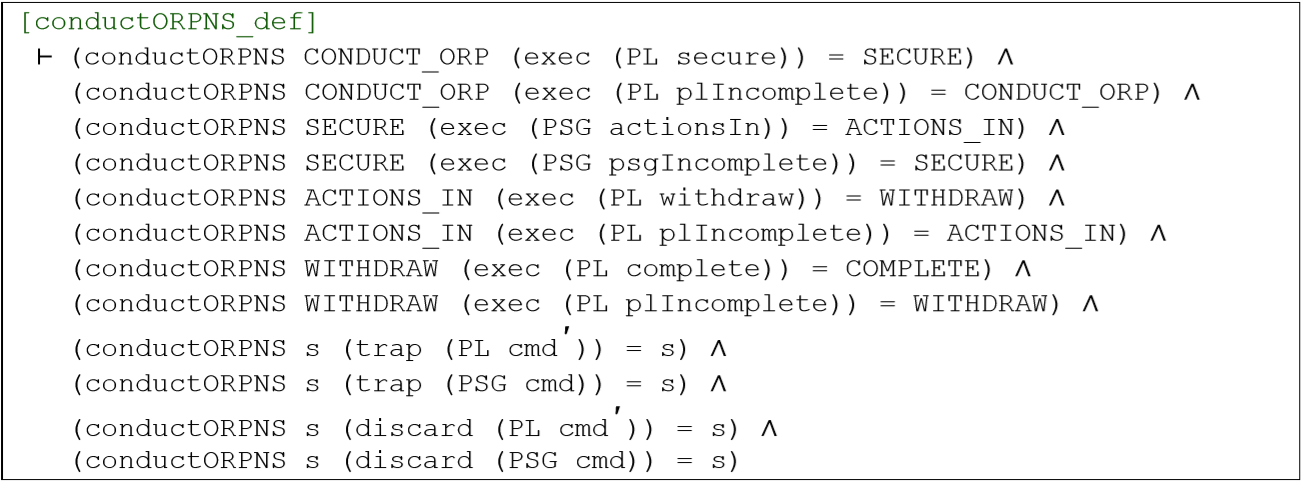
\includegraphics[width=0.8\linewidth]{conductORPNS.PNG}
\end{figure}

 In the line "CONDUCT_ORP (exec (PL secure)) = SECURE)", CONDUCT_ORP was the initial state,
  (exec (PL secure)) was the transition type applied to the command "secure", and SECURE was the
  state of the \textit{secure} state machine if the command was executed.  In the line,
  "s (trap (PL cmd′)) = s, "s" was a variable for any valid state, (trap (PL cmd)) was the
  transition type applied to the command "cmd", and "s" was the state after the trap command
  was applied.  Note that trapped transitions were not allowed and the state machine did not
  change states.  The \textit{discard} transition type followed a similar logic.  PL and PSG
  were constructors that helped HOL determine what type of command followed. PL indicated that
  the command was a Platoon Leader command and PSG indicated that the command was a Platoon Sergeant command.\\
  
 Next output functions followed a similar logic.  Although, we did not focus on
  outputs for our \textit{secure} state machines, they were required to parameterize ssm11
  and ssm.  The next output function for the secure state machines described an initial state,
  a transition type applied to a command, and the output that resulted.  In the definition of
  the next output function in the text box above, imagine replacing the final states with an
  output.    The next output function for the same \textit{secure} state machine described
  above was shown in the text box below.   The pattern should be evident.\\
  
  \begin{figure}[h]
  \centering
  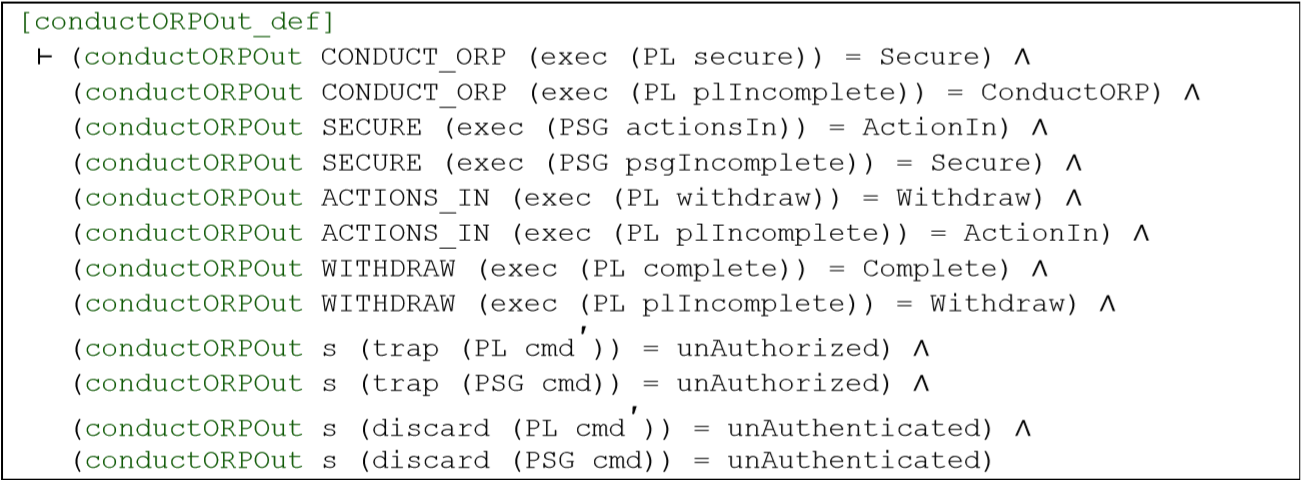
\includegraphics[width=0.8\linewidth]{conductORPOut.PNG}
\end{figure}


\subsection{states, commands/inputs, outputs, and Principals}
\label{sec:stat-comm-outp}


\begin{itemize}
  \item The basic datatypes were defined for all theories in the OMNIType Theory (HOL/OMNITypeScrip.sml).
  These were \textit{state, command, output, and principal}.   In their definitions, each of these
  contained a constructor followed by a state-level defined datatype.   An example of the
  \textit{command} datatype definition in the OMNIType Theory was shown below.\\
  
  \begin{figure}[h]
  \centering
  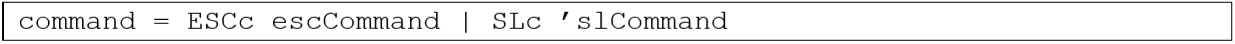
\includegraphics[width=0.8\linewidth]{command.PNG}
\end{figure}

 \item \textit{SLc} was the constructor for a command of type \textit{slCommand}.  The \textit{ESCc escCommand}
  was not verified in this project.  The escape states and commands were designed to allow abortion of the
  operation.  The idea is that certain conditions, such as contact with enemy, required escape from any state.
  These states were not verified in HOL, but they were retained in the OMNIType Theory for future inclusion
  into the state machines.\\
  
  \item The other OMNIType datatypes were shown below.\\
  
  \begin{figure}[h]
  \centering
  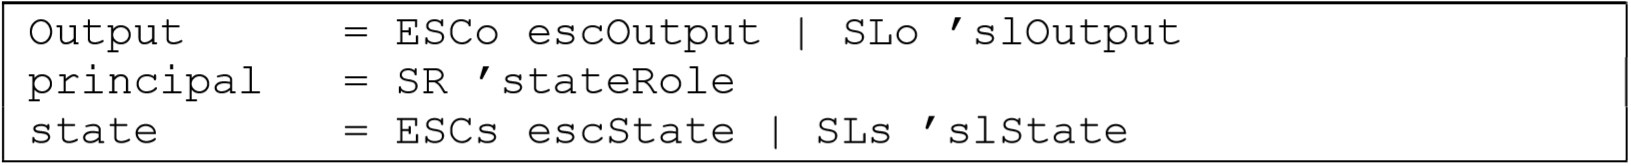
\includegraphics[width=0.65\linewidth]{output.PNG}
\end{figure}

 \item In \textit{secure} state machines, \textit{command, state, ourput,} and \textit{principal}
  were defined with the specific commands for that state.  For example, the text box below shows
  the definition of these datatypes for a \textit{secure} state machine that used only one principal.
  \begin{figure}[h]
  \centering
  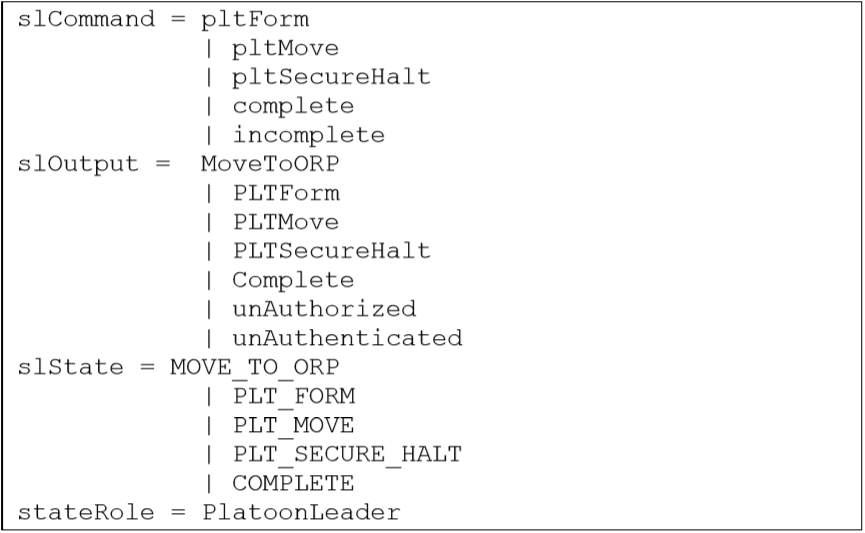
\includegraphics[width=0.6\linewidth]{slCommand.PNG}
\end{figure}

 \item For \textit{secure} state machines with multiple principals, it was easier to define
  commands that each principal could issue separately from one another.  Therefore, the Platoon
  Leader could make Platoon Leader commands \textit{(plCommand)} and the Platoon Sergeants could
  make Platoon Sergeant commands \textit{(psgCommand)}.  \textit{stateRole, slOutput,} and
  \textit{slState} did not require separate commands.  An example of these datatype definitions
  for \textit{slCommand} was shown below.
  
  \begin{figure}[h]
  \centering
  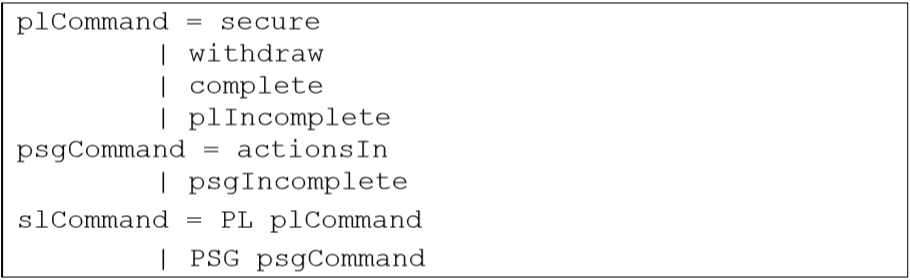
\includegraphics[width=0.6\linewidth]{plCommand.PNG}
\end{figure}

\end{itemize}

\section{Configurations}
\label{sec:configurations}

State machines are defined by their next state and next output functions.  But, \textit{secure} state
machines also require principals, authentication verification techniques, and authorization lists.  In
addition, to the next state and next output functions, our \textit{secure} state machines were defined
by configurations.  These configurations included the following entities:
\begin{itemize}
\item Authentication Test Function
\item State Interpretation Function
\item Security Context List
\item Input
\item Current State
\item Output\\
  \end{itemize}
  
\subsection{Authentication Test Function}
\label{sec:auth-test-funct}

  This function tests the principals for proper authentication.  As described above,
  authentication for this project was assumed to be done by familiarity.  The authentication
  test function returned true if the authentication was verified and false otherwise.
  
\subsection{State Interpretation Function (state specific rules)}
\label{sec:state-interpr-funct}


  The state interpretation function defined logical rules that were specific to each state.
  For our project, the state interpretation function was not used.  However, it was required
  for the configurations.  Thus, stateInterp function was defined to return the trivial value
  TT, the ACL logical value for true.
  
\subsection{Security Context List}
\label{sec:secur-cont-list}

  The security context consisted of the policies regarding \textit{which} principal had authority
  to make \textit{which} commands. The security context was thus a list of ACL formulas of the form
  "SomePrincipal controls someCommand", where \textit{controls} is the ACL logical expression of authority.
  
\subsection{Input}
\label{sec:input}

   The input was of the form "somePrincipal says someCommand."  \textit{says} is the ACL
    logical expression of a request.   In this case, \textit{somePrincipal} is requesting to
    execute \textit{someCommand}.  In ssm11, the input was a single ACL \textit{says} statement.
    In the ssm, the input was a list of these statements:  ["somePrincipal1 says someCommand1",
    "somePrincipal2 says someCommand2", ...].\\
    
   In the configurations and the theorems, the input was represented as an input stream.
    The input stream was expressed in HOL as a list.  The list was of the form firstElement::remainderOfList.
    The "::" is the "cons" operation and it separated the first list element from the remainder of the
    list.  The first element of the list was the ACL request: "somePrincipal says someCommand" in the
    case of ssm11 and the corresponding list in the case of ssm.   The input for ssm was thus a list of
    lists.  The remainder of the list was simply a variable for our theorems.  This variable was typically
    named \textit{ins}.  Thus, an input in our configurations had the following form.\\
    
    \begin{figure}[h]
  \centering
  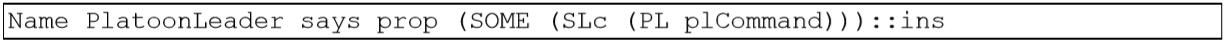
\includegraphics[width=0.8\linewidth]{name.PNG}
\end{figure}

 The left side of the "::" operator was the strongly-typed version of "somePrincipal says
  someCommand."  \textit{Name} was the ACL constructor for a principal.  The principal in this
  example was \textit{PlatoonLeader}. \textit{prop} was the ACL constructor for a proposition.
  In our example, propositions were commands.  \textit{SOME} told HOL that what follows was some
  command (rather than NONE).   \textit{ins} followed the "::" operator and represented the tail
  of the list.

\subsection{Current State}
\label{sec:current-state}

The current state was the current state.  Nothing special here.

\subsection{Output}
\label{sec:output}

Outputs were not used, but were defined in order to use ssm11 and ssm.  They were often represented
with the variable \textit{out, outs,} or \textit{output}.  Outputs in configurations were also streams.
After a transition from one state to another was executed (or trapped or discarded), the resulting
output was "cons-ed" onto the previous output stream.  This looked like \textit{newOutput::outputStream}.

\section{Theorems}
\label{sec:theorems}

 For this project, there was one primary theorem.  It proved that a transition was executed if
  and only if the proper authentication and authorization were verified.  This was sufficient to
  satisfy the principals of complete mediation.  It was proved for each principal issuing commands.
  Thus, for secure state machines with two principals, one theorem was proved for each principal.
  An example of this theorem was shown below.\\
  
\begin{figure}[h]
  \centering
  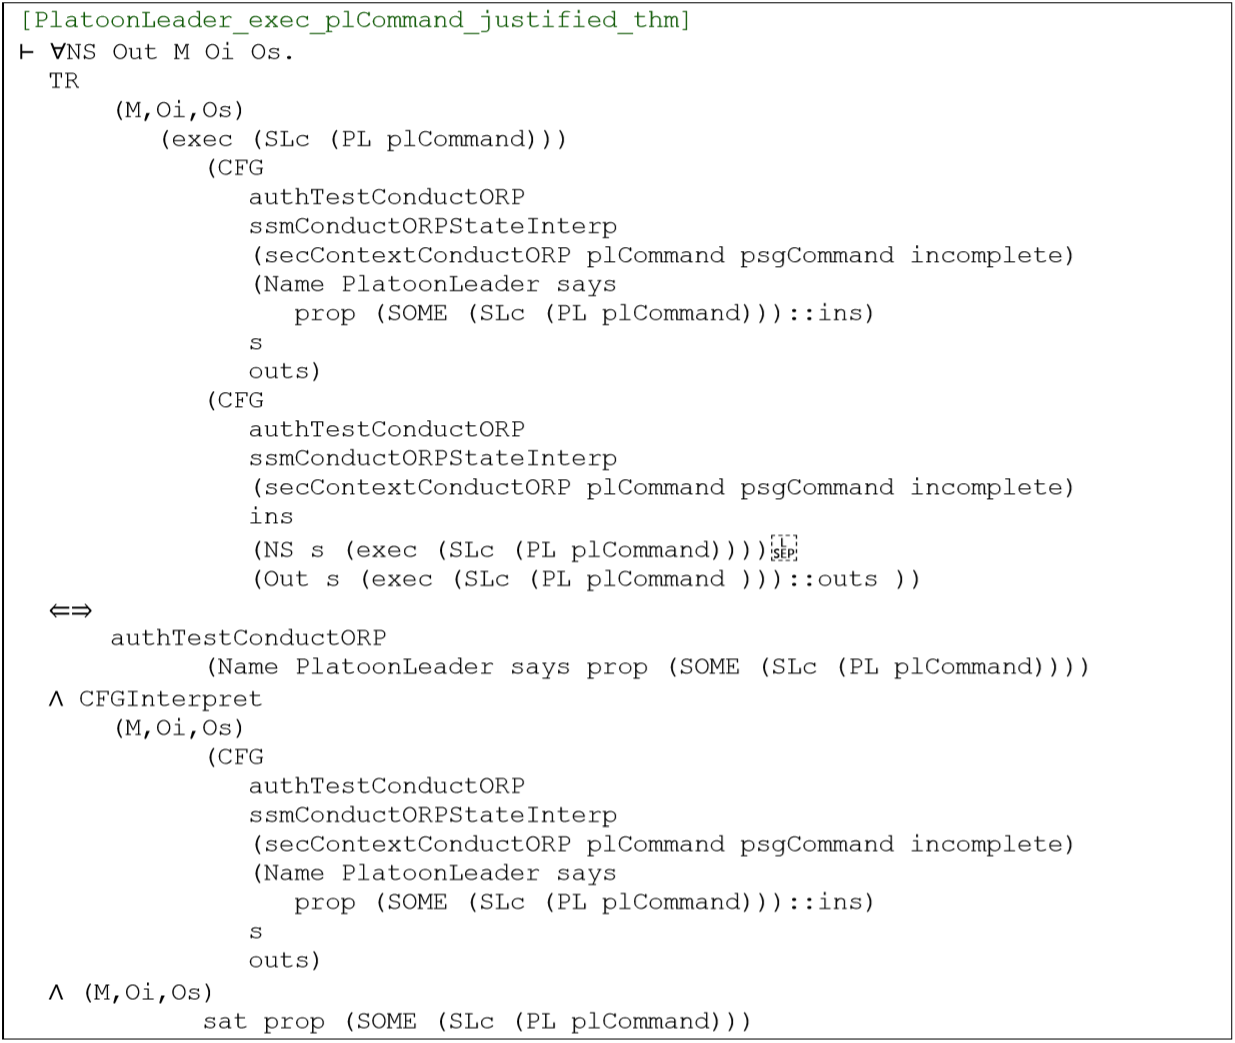
\includegraphics[width=0.8\linewidth]{PlatoonLeader.PNG}
\end{figure}

 The name of this theorem was \textit{PlatoonLeader_exec_plCommand_justified_thm}.  The theorem
  justified executing transitions wherein the \textit{PlatoonLeader} issued commands of type \textit{plCommand}.
  The next line stated that this theorem was valid for all next state (NS) functions, output (Out),
  and Kripke Structures (M, Oi, Os).  (Kripke Structures are explained in the text book.  Kripke
  Structures were not defined for the patrol base operations.  But, they are part of the ACL and are
  required for application of the ACL theories.)
  \\
 \textit{TR} was the Transition Relation function.  It took as input a Kripke Structure,
  a transition type with a command, and an initial configuration.  It returned a final configuration.
  In this example, the transition type with the commands was \textit{(exec (SLc (PL plCommand)))}.
  This told HOL that the transition from the initial to final state was executed for commands of type
  \textit{plCommand}.\\
  
 The initial configuration was preceded by the constructor \textit{CFG}.  The authentication
  test function was named \textit{authTestConductORP}.  The state interpretation function was named
  \textit{ssmConductORPStateInterp}.  The security context list was named \textit{secContextConductORP}.
  This took three parameters: \textit{plCommand, psgCommand} and \textit{incomplete}.  These were the
  allowable command datatypes.  The input stream was \textit{Name PlatoonLeader says prop (SOME (SLc
    (PL plCommand)))::ins}. The first element of this stream (before the ":") was the ACL request to
  change states.  The other part the input stream was the variable \textit{ins}.  The current state
  was \textit{s}.  The output was \textit{outs}.\\
  
 The final configuration was also preceded with the constructor \textit{CFG}.  In this final
  configuration, the first three elements \textit{authTestConductORP, ssmConductORPStateInterp,} and
  \textit{secContextConductORP}  were unchanged.  The input stream changed by pealing-off the first
  element.  \textit{ins} remained.  The state changed by applying the next state \textit{(NS)} function.
  The function call was \textit{(NS s exec (SOME (SLc (PL plCommand)))}.  Similarly, the output changed
  by adding the initial output to the output stream. The function call was onto the front of the list:
  \textit{(OUT s exec (SOME (SLc (PL plCommand)))::outs)}.\\
  
 In summary, this first part of the biconditional stated that the result of executing the command
  \textit{plCommand} with the transition type \textit{exec} was a transition from the initial configuration
  to the final configuration described above.\\
  
 The second part of the biconditional checked the authorization and authentication of the principal
  issuing the request.  It was a conjunction of three parts.  For the first part, the \textit{authTestConductORP}
  had one parameter, the input request \textit{Name PlatoonLeader says prop (SOME (SLc (PL plCommand))).
    authTestConductORP} returned true if \textit{PlatoonLeader} was authenticated on \textit{plCommands}
  and returned false otherwise.\\
  
 The third part verified that the command/proposition \textit{prop (SOME (SLc (PL plCommand))}
 satisfied the Kripke structure.  For this project, this meant that the command was justified.\\
 
 In summary, the first and last part of the biconditional proved that the transition from initial
  state to final state was executed if and only if the \textit{PlatoonLeader} issued a \textit{plCommand}
  and the \textit{PlatoonLeader} was authorized on the \textit{plCommand}.\\
  
 HOL was used to prove \textit{PlatoonLeader_exec_plCommand_justified_thm}.  To prove this theorem,
  we parameterized an ssm11 theorem named \textit{TR_exec_cmd_rule} was proved in ssm11.  Parameterization
  is why we used ssm11.  The \textit{TR_exec_cmd_rule}  was used with the ISPECL rule in HOL to replace the
  variables in \textit{TR_exec_cmd_rule}  with the variables used in \textit{PlatoonLeader_exec_plCommand_justified_thm}.
  An example of the ISPECL rule used to prove \textit{PlatoonLeader_exec_plCommand_justified_thm} was shown below.\\
  
  \begin{figure}[h]
  \centering
  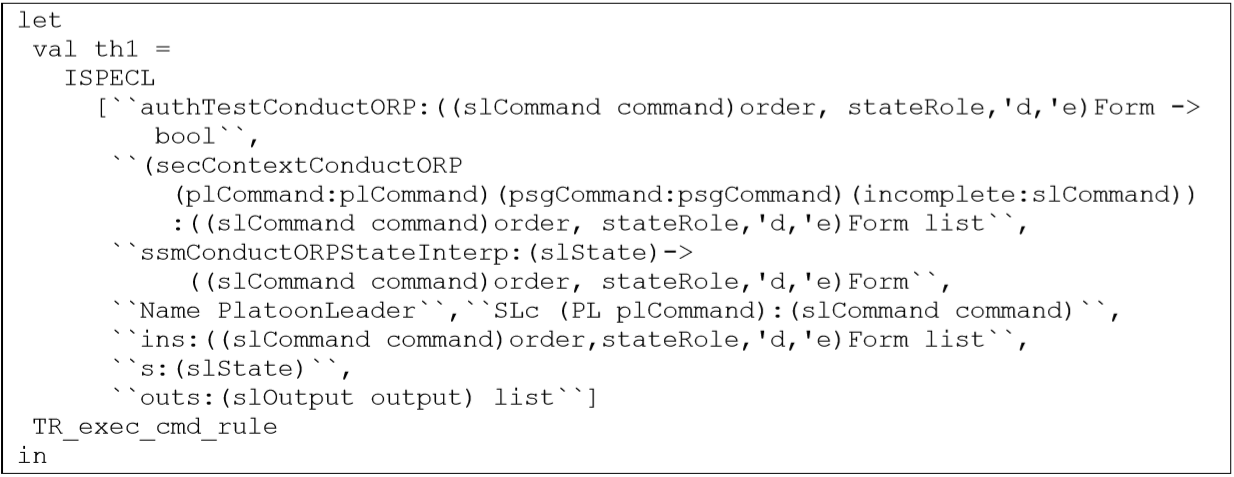
\includegraphics[width=0.8\linewidth]{th1.PNG}
\end{figure}

 HOL needed the double back-quotes ` ` to recognize terms.  The excess "junk" that followed
  each variable (or parameter) was the typing.  Remember HOL was a strongly-typed language.  Thus,
  the first parameter was \textit{authTestConductORP}.  The second was \textit{secContextConductORP}.
  The third was the principal \textit{Name PlatoonLeader}.  The fourth parameter was the command
  \textit{SLc (PL plCommand)}.  The fifth was the input stream (without the first element)
  \textit{ins}.  The sixth was the state \textit{s}.  The seventh was the output stream
  \textit{outs}.  The \textit{let} and \textit{in} statements were part of the proof construct.
  \textit{val th1 =} essentially set-up this specialized version of \textit{TR_exec_cmd_rule} and
  temporarily saved it as \textit{th1}.\\
  
 To prove \textit{PlatoonLeader_exec_plCommand_justified_thm} we needed one more theorem,
  actually a lemma.  This lemma proved the second and third part of the second half of the biconditional.
  It was shown below.\\
  
  \begin{figure}[h]
  \centering
  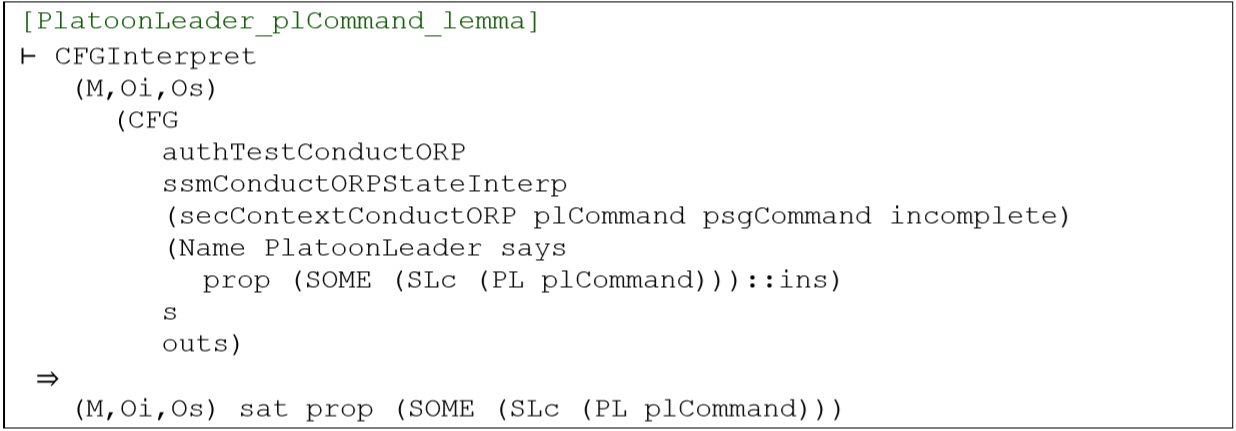
\includegraphics[width=0.8\linewidth]{PlatoonLeader2.PNG}
\end{figure}

 \textit{PlatoonLeader_plCommand_lemma} proved that the initial configuration justified the
  proposition.  To convince HOL the lemma was true, we directed HOL to look at several definitions:
  the \textit{authTestConductORP}, which stated that the \textit{PlatoonLeader} was authenticated
  on the input; the \textit{ssmConductORPStateInterp}, which was defaulted to TT (ACL for true);
  and the \textit{secContextConductORP}, which stated that \textit{PlatoonLeader} controls the input.
  With this information reformatted by the \textit{CFGInterpret} function, HOL used the following
  ACL rule to justify the proposition.\\
  
  \begin{figure}[h]
  \centering
  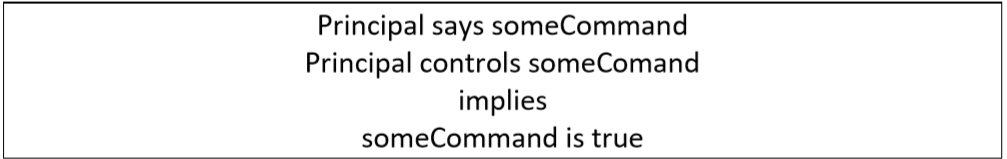
\includegraphics[width=0.6\linewidth]{principal.PNG}
\end{figure}



\section{Parameterizable Secure State Machines}
\label{sec:param-secure-state}


\subsection{ssm11}
\label{sec:ssm11-1}

 ssm11 was the initial \textit{secure} state machine that was verified before the
  start of this project.  The name means "secure state machine version 1.1".  The original
  version was ssm1.  ssm1 was modified for this project.  The modifications were minor.
  They included a change of name from \textit{inst} in the original to order in ssm11.
  Also, \textit{discard} transitions were modified to act like the \textit{trap} transitions.
  Although, neither \textit{trap} nor \textit{discard} were the focus of this project.\\
  
 The reason ssm1 was used was because it represented a \textit{secure} state machine
  theory that was already implemented in HOL and that had already been verified.  In addition,
  it was parameterizable.  This meant that we could replace variables in ssm1 (ssm11 and ssm,
  see later) with the parameters in our state-level \textit{secure} state machines.  Thus, to
  prove that our \textit{secure} state machines followed the principles of complete mediation,
  we only needed to parameterize the \textit{TR_exec_cmd_rule} proved in ssm11 using the SPECL
  function (as described above in the \underline{Theorems} section).\\
  
 The ssm11 required a major overhaul to accommodate multiple input statements.  The
  overhauled version was named ssm because the overhaul was significant enough to warrant it
  replacing all future versions of ssm11 (and ssm1).  However, we did not replace versions of
  ssm11 in this project if they were verified before the overhaul.  Any future \textit{secure}
  state machines would use the new ssm, such as sub-sub-level \textit{secure} state machines
  (if time allowed).  We did apply the new ssm to the ssmPlanPB secure state machine.  We
  called this new version ssmNewPlanPB.  The older version that used ssm11, ssmPlanPB, may
  have been removed from the project folders by the time this paper was complete.\\
  
 The sections below clarified areas of the ssm11.\\

  
\subsubsection{Configurations}
\label{sec:configurations-1}

  Configurations were defined in ssm11 and implemented in the state-level \textit{secure} state
  machines.  Configurations were described above.

  
\subsubsection{CFGInterpret Function}
\label{sec:cfgint-funct}

  \textit{CFGInterpret} condensed the configuration into a "satisfies" list that was valid for all
  \textit{(M, Oi, Os)}.  In ACL, "satisfies" meant that some rule was valid for a given
  \textit{(M, Oi, Os)}.  \textit{CFGInterpret} proved that the theorem was true for ALL
  \textit{(M,Oi,Os)}.  Therefore, it was not necessary to specify such a structure.  For
  more information on "satisfies" and \textit{(M,Oi,Os)}, see the text book
  \textit{Access Control, Security, and Trust: A Logical Approach}.  The definition of
  \textit{CFGInterpret} was shown in the text box below.\\
  
  \begin{figure}[h]
  \centering
  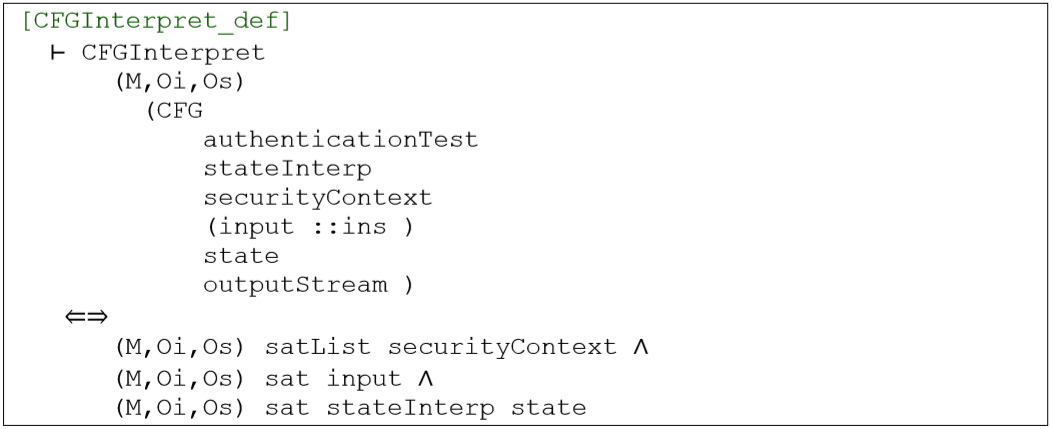
\includegraphics[width=0.8\linewidth]{CFGInterpret.PNG}
\end{figure}

 This was a biconditional.  The top part was the configuration.   The part following
  the $\Leftarrow \Rightarrow$ symbol was the "sat" statements that included the security context, the input,
  and the result of the state interpretation function applied to the state.


 \subsubsection{TR\textunderscore rules, TR\textunderscore cases, TR\textunderscore ind}
\label{sec:trtext-rules-trtext}


  \textit{TR_rules, TR_cases, TR_ind} described the \textit{secure} state machine \textit{TR}
  (Transition Relations).  The text box below showed the definition.  (Note that this definition
  looks different from many of the others in this document because this definition was taken from
  the ssm11Script.sml file whereas the others were taken from the EmitTeX generated pretty-printed files.)\\\\\\
  \\\\\\\\\\\\
  \begin{figure}[h!]
  \centering
  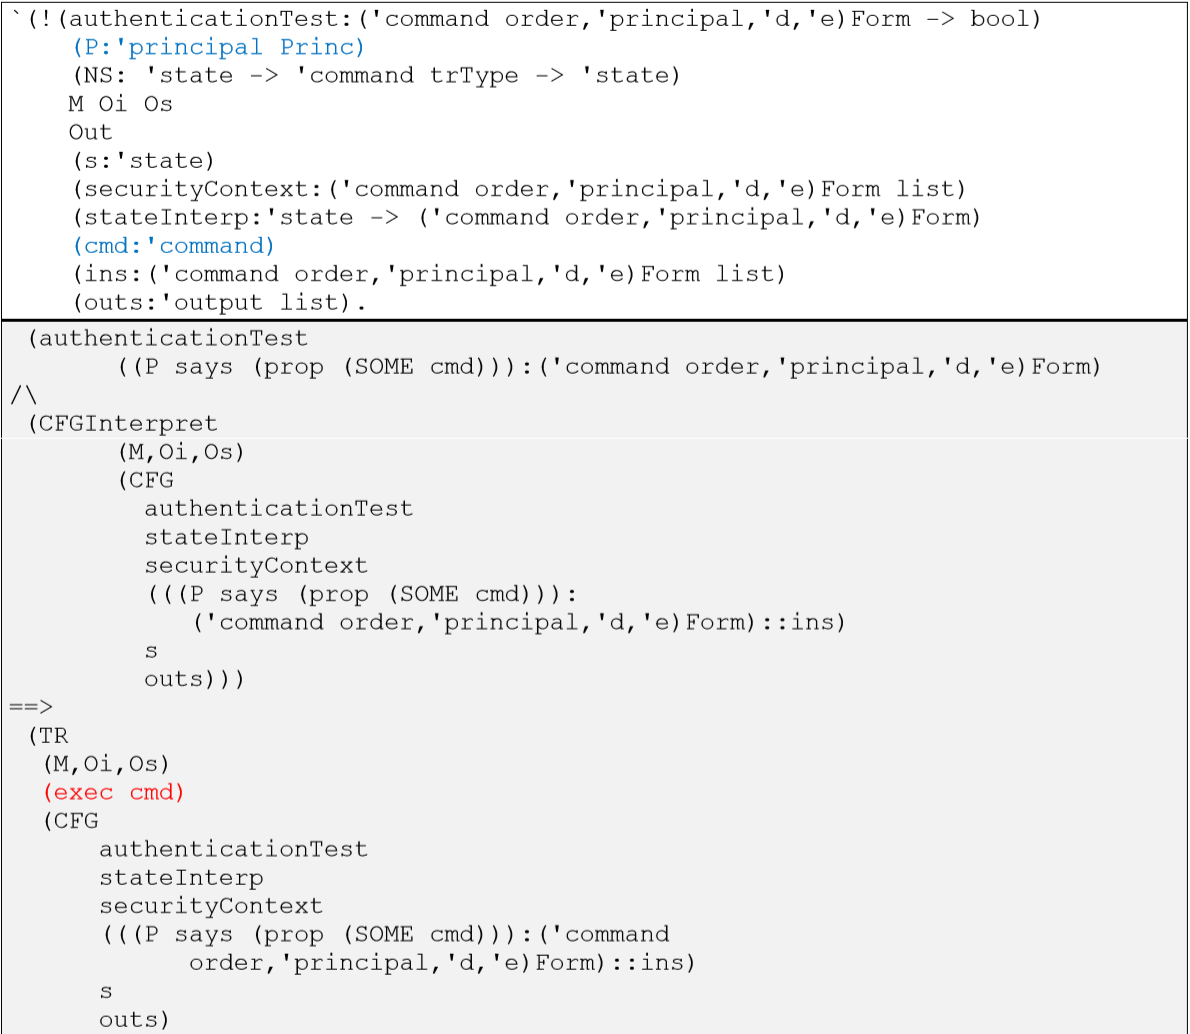
\includegraphics[width=0.8\linewidth]{TR1.PNG}
\end{figure}

\begin{figure}[h!]
  \centering
  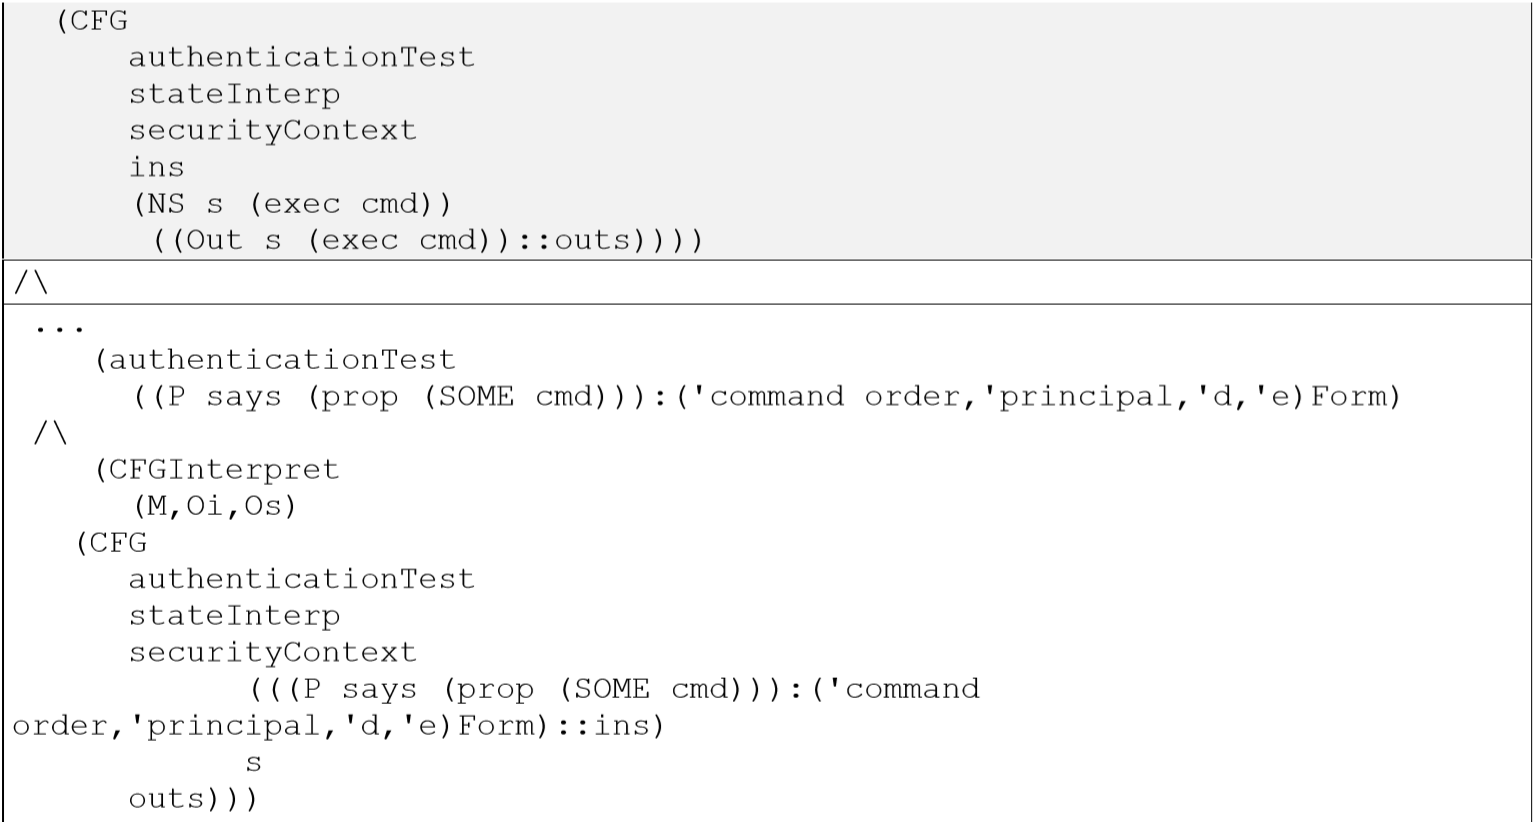
\includegraphics[width=0.8\linewidth]{TR2.PNG}
\end{figure}
\begin{figure}[h!]
  \centering
  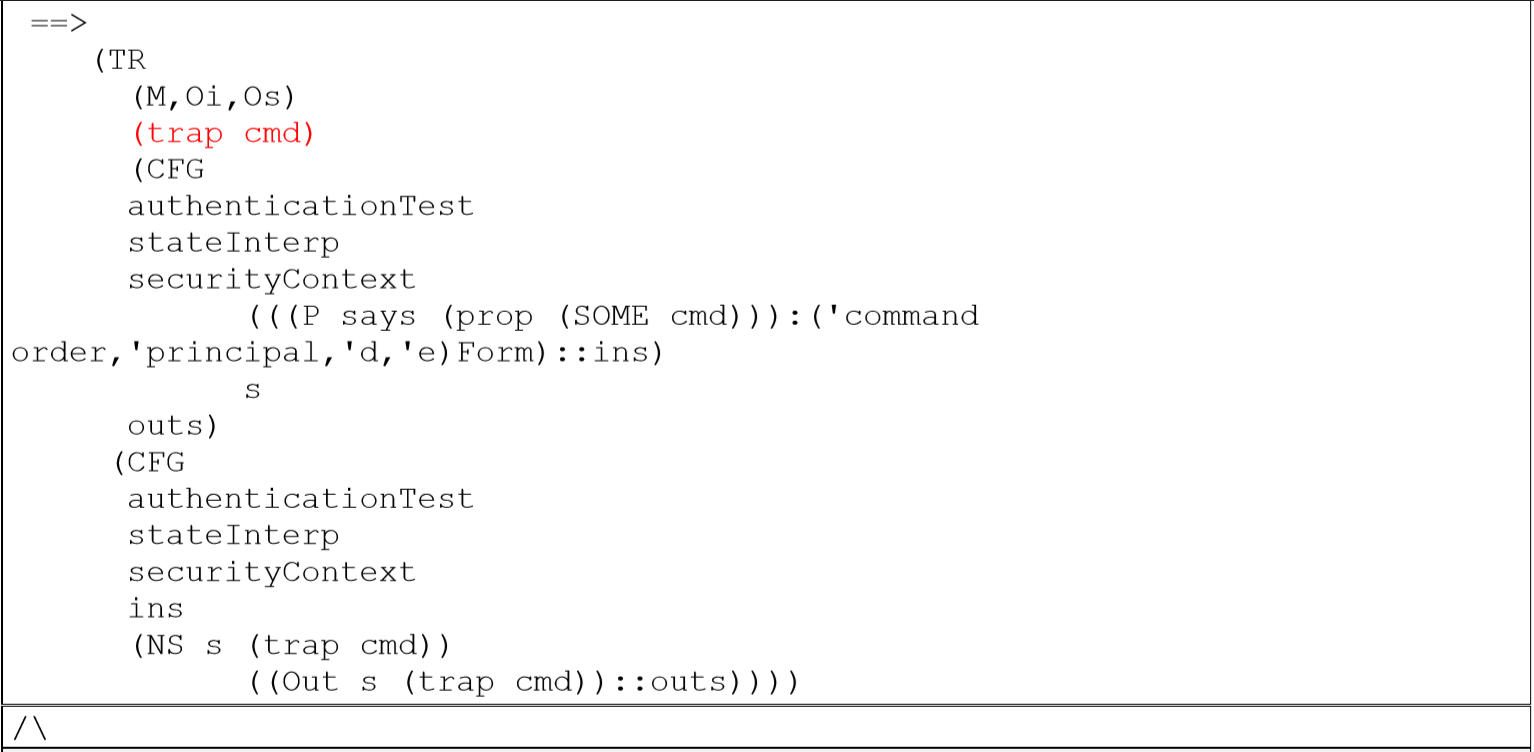
\includegraphics[width=0.8\linewidth]{TR3.PNG}
\end{figure}
\begin{figure}[h!]
  \centering
  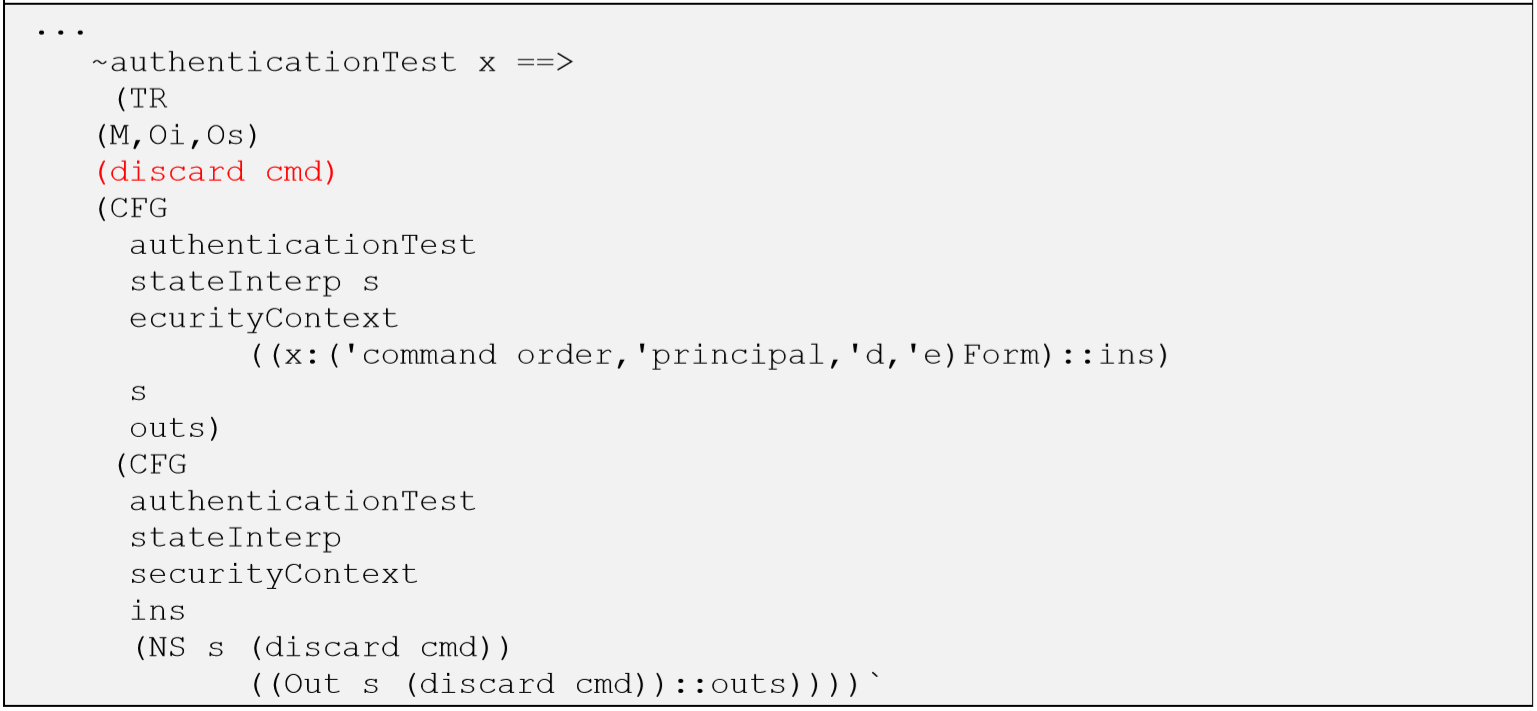
\includegraphics[width=0.8\linewidth]{TR4.PNG}
\end{figure}
 The above code was modified somewhat to make it easier to read in this document.
  The lines and highlighting distinguished logical sections of the code.  The top section
  stated that what followed was true for all the pertinent variables in the list.  This
  section was repeated two additional times in the code.  For brevity, it was repeated as "..."\\
  
 The parts in \textcolor{cyan}{blue} became problematic and prompted the overhaul of ssm11 to ssm.
  This was discussed further in the appropriate section describing ssm.  The text in red
  were the transition types with the commands.  Notice that there was a separate transition
  type for each of the major blocks (save for the top block).  The blocks were also similar.
  They described the rules for one transition type denoted in \textcolor{red}{red}.\\
  
 The reader should have noticed the similarity of the definition above to
  \textit{PlatoonLeader_exec_plCommand_justified_thm} in the \underline{Theorems} section.
  In the case here, the conclusion and premise were reversed.  In addition, only the first
  and second part of the conclusion were present.  Therefore, the first part of each section
  defined the authentication \textit{(authenticationText)} and the authorization
  (\textit{CFGInterpret} applied to the configuration).  The conclusion that followed
  the "==$>$" symbol defined the Transition Relation \textit{TR}.\\
  
 The first major block (lightly shaded)  described the Transition Relation for
  the \textit{exec} transition type.  The second major block described the Transition Relation for
  the \textit{trap} translation type.  The last block described the Transition Relation for the
  discard transition type.\\


\subsubsection{TR\textunderscore exec\textunderscore cmd\textunderscore rule}
\label{sec:trtext-exect-cmdt}


  \textit{TR_exec_cmd_rule} proved that a transition between states occurred if and only if
    the principal was authenticated and authorized on the executed command.  The theorem was shown below.\\
    
  \begin{figure}[h]
  \centering
  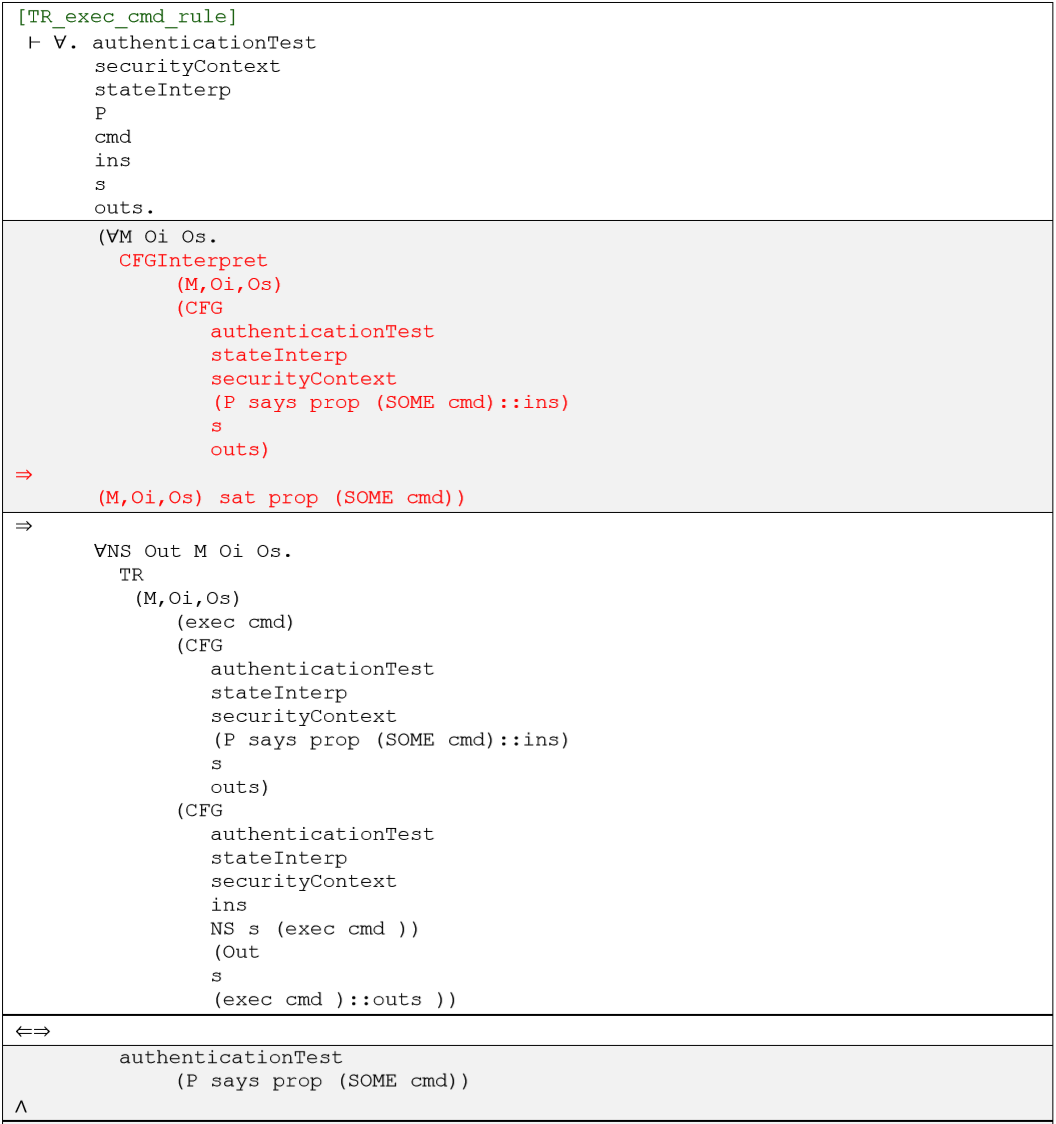
\includegraphics[width=0.8\linewidth]{TRexec.PNG}
\end{figure}
\begin{figure}[h!]
  \centering
  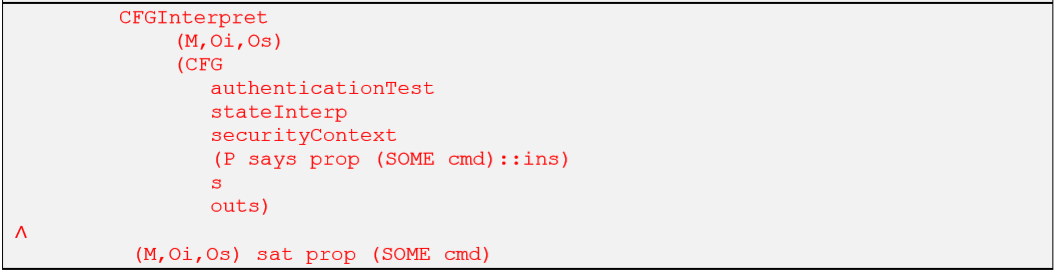
\includegraphics[width=0.8\linewidth]{TRexec2.PNG}
\end{figure}

 Notice the greater similarity of this code to \textit{PlatoonLeader_exec_plCommand_justified_thm}.
  That's because \textit{PlatoonLeader_exec_plCommand_justified_thm} parameterized \textit{TR_exec_cmd_rule}.
  The first part of this theorem was the "for all" list of parameters.  The red-text sections were essentially
  the parameterizable version of \textit{PlatoonLeader_plCommand_lemma}.  They proved the principal was
  authorized and authenticated on the exec transition type.  The non-highlighted text was the Transition Relations.\\
  
 An expection of TR_exec_cmd_rule, \textit{PlatoonLeader_exec_plCommand_justified_thm},
 and \textit{PlatoonLeader_plCommand_lemma} should have revealed the similarity.\\
 
 
\subsubsection{TR-trap-cmd-rule}
\label{sec:tr-trap-cmd}


  \textit{TR_trap_cmd_rule} was similar to \textit{TR_exex_cmd_rule}.  There were two differences.
  The first difference was that \textit{exec cmd} was replaced \textit{trap cmd}.  The second difference
  was that (M,Oi,Os) sat prop (SOME cmd) was replaced with that (M,Oi,Os) sat prop  NONE.  The
  highlighted code in the text box below showed this second difference.\\
  
  \begin{figure}[h]
  \centering
  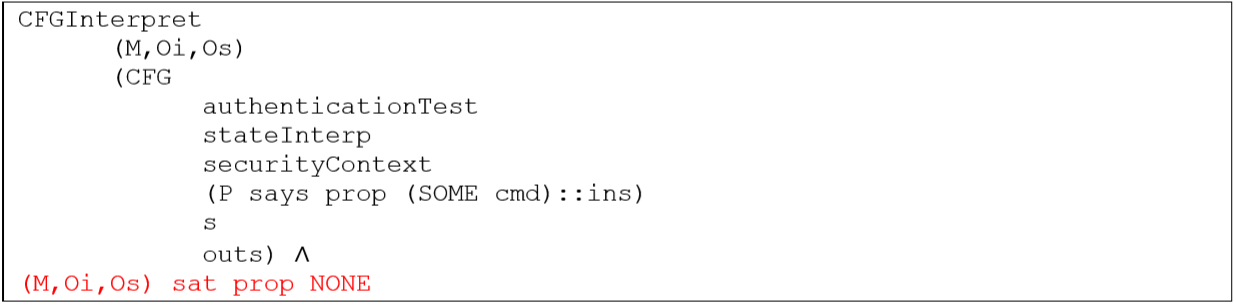
\includegraphics[width=0.75\linewidth]{CFGInterpret2.PNG}
\end{figure}


\subsubsection{TR-discard-cmd-rule}
\label{sec:tr-discard-cmd}

  \textit{TR_discard_cmd_rule} proved that the \textit{discard cmd} was applied to the state machine
  if and only if the authentication test failed.  (\textit{~authentication x}).  That code was shown below.\\
  
  \begin{figure}[h]
  \centering
  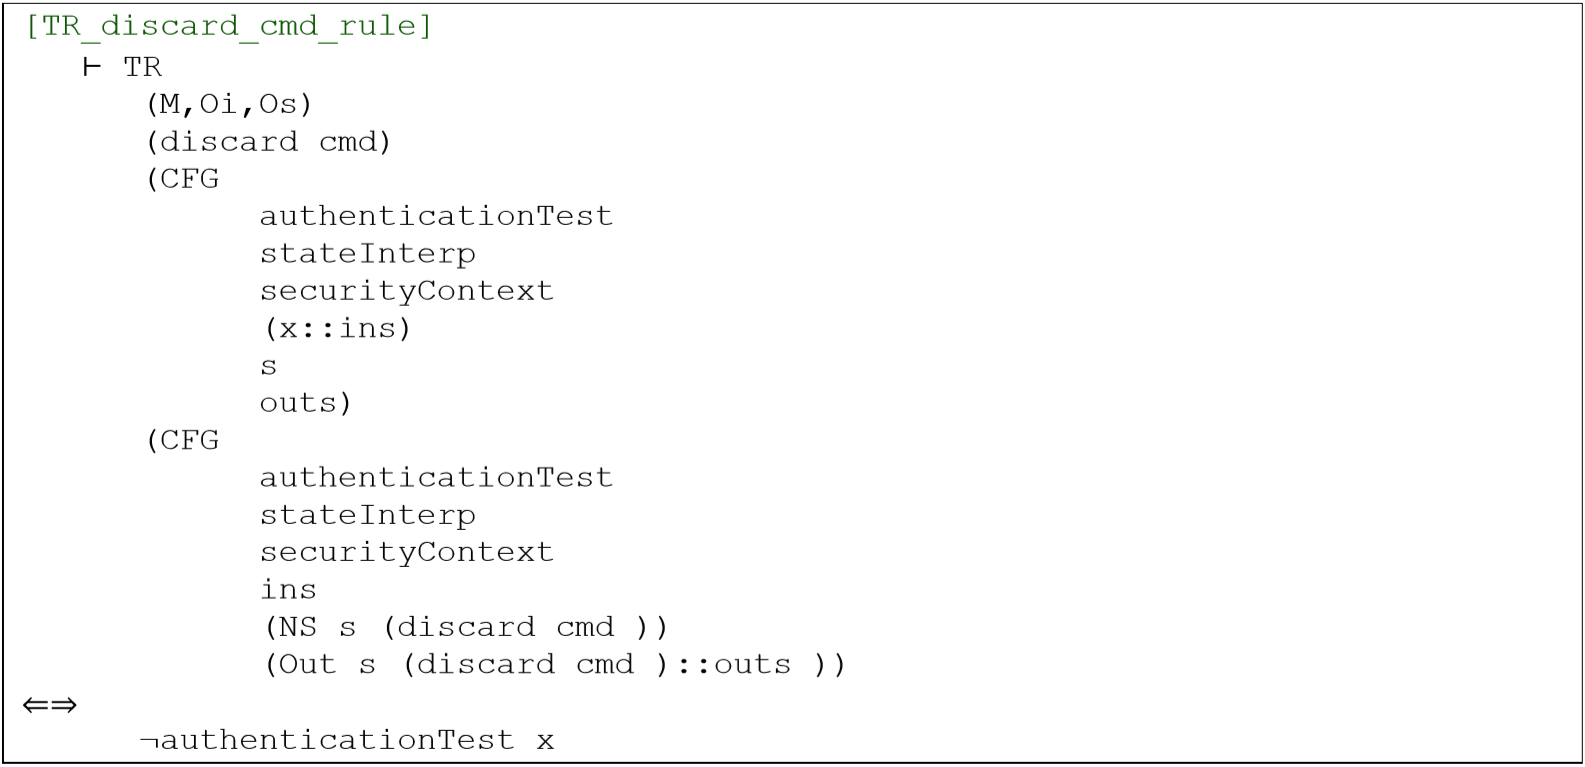
\includegraphics[width=0.75\linewidth]{TRdiscard.PNG}
\end{figure}

 Other theorems and datatypes in the ssm11 supported the main theorems and datatypes described above.
  The complete list of the theorems was shown in the EmitTeX pretty-printed code in the appendix .\\


\subsection{ssm}
\label{sec:ssm-1}

 ssm was an overhaul of ssm1.  There were two basic changes made to ssm11.  The first was the
  elimination of the \textit{order} type.  In the ssm11, this served as an option type.  But, HOL
  already had a predefined option type with supporting theories.  Therefore, we used the HOL built
  in option type found in optionTheory.\\
  
 The second change was the main reason for the overhaul.  The overhaul added functionality
  to the ssm11 theory.  This functionality allowed for an input list of ACL formulas rather than a
  single input formula.  For example, the following would be an appropriate input for ssm11.\\
  
  \begin{figure}[h]
  \centering
  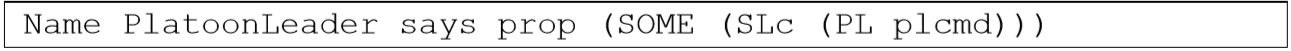
\includegraphics[width=0.8\linewidth]{name2.PNG}
\end{figure}

 This input was a command from the PlatoonLeader.  But, single commands of this type were not
  sufficient for more complex secure state machines.  For more complex machines, several requests were
  required for a transition.  For example, in the ssmPlanPB \textit{secure} state machine, to transition
  from the WARNO state to the COMPLETE_PLAN state, the machine had to pass through three other states
  first: TENTATIVE_PLAN, INITIATE_MOVEMENT, and REON.  These three states were executed in any order.
  But, all three had to be executed before transitioning to COMPLETE_PLAN.  To do this in, we
  transitioned directly from the WARNO state to the COMPLETE_PLAN state.  But, we changed the input
  for transition to be a list wherein the appropriate principals for each of the three non-sequential
  states and the WARNO state had to issue the following commands:
  \begin{itemize}
  \item PlatoonLeader says tentativePlan,
   \item  PlatoonSergeant says initiateMovement, 
   \item PlatoonLeader says recon, 
   \item PlatoonLeader says completePlan
   \end{itemize}
   If all four commands were issued, then HOL was instructed to allow the transition. \\
   
    This type of list of multiple inputs allowed for the variation needed to represent the
     more complex secure state machines in the project.  Of course, this type of input list was not
     permitted by ssm11.  The problem was in the description of the \textit{TR_rules, TR_cases, TR_ind}.
     The problem code was repeated in the blue text in the following excerpt from \textit{TR_rules, TR_cases, TR_ind}.\\
     
\begin{figure}[h]
  \centering
  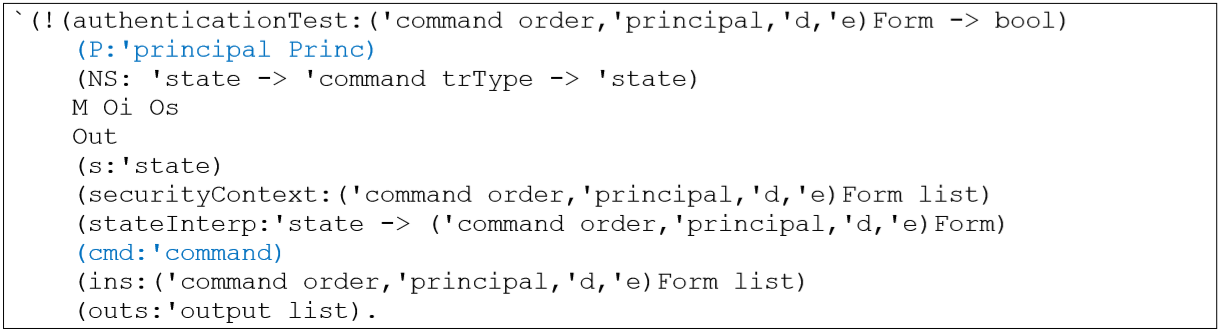
\includegraphics[width=0.8\linewidth]{authenticationTest.PNG}
\end{figure}

 The code above was intended to be parameterized with the name of a principal and the type of
  command.  However, there were multiple principals with multiple commands.  The entire Transition
  Relations had to be redefined to accommodate this.  The accommodation required significant modification
  and verification of the code.  But, the improvements were worth the wait.  \\
  
  What follows explained where ssm differed from ssm11.

\subsubsection{Configurations}
\label{sec:configurations-2}

  Configurations did not change.

\subsubsection{Additional Functions}
\label{sec:additional-functions}

   Several additional functions were added to accommodate the overhaul. Those functions and
   there were explained below.\\

   \begin{itemize}
   
   \item \underline{authenticationTest}\\
     \textit{authenticationTest} was not a new function.  But, it's use was modified somewhat in ssm.
      The \textit{authenticationTest} function in ssm11 took an input stream as a parameter and returned
      true or false.  It was defined in each of the \textit{secure} state machines that parameterized ssm11.
      The definition consisted of a conjunction of ACL formulas of the form "somePricnipal says someCommand = T".
      The input stream was also of the form needed by ssm11, in particular singleACLRequest::remainderOfList.
      But, the input for ssm was not an input stream consisting of ACL formulas.  It was an input stream
      consisting of ACL formula \textit{lists}.\\
      
     The \textit{authenticationTest} reduced the input list to a single T or F boolean value that our
      theorems needed to verify the authentication of the input.  \textit{authenticationTest} took two
      parameters \textit{elementTest x}.  \textit{elementTest} was a function and \textit{x} was the input list.
      elementTest in ssm behaved exactly the same as \textit{authenticationTest} in ssm11.  It took a single
      ACL formula as input.  It returned true if the input was authenticated and false otherwise.
      \textit{authenticationTest} in ssm did two things.  First, it mapped the \textit{elementTest} onto each
      element in the input list \textit{x}. The result was a list of T or F boolean values.
      \textit{authenticationTest} then "folded" the T boolean value onto this list.  The result in this
      case was T if all the elements in the list were true and false otherwise.  The code for
      \textit{authenticationTest} in ssm was shown below.\\
      
\begin{figure}[h]
  \centering
  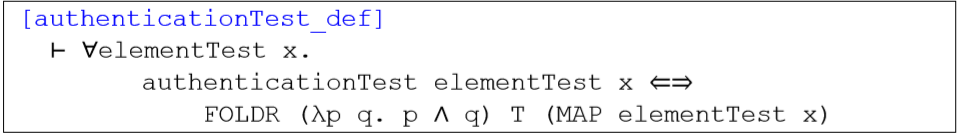
\includegraphics[width=0.6\linewidth]{authenticationTest2.PNG}
\end{figure}

 The \textit{authenticationTest} reduced the input list to a single T or F boolean value that our
  theorems needed to verify the authentication of the input.\\


 \item \underline{extractCommand}\\
  \textit{extractCommand} took an ACL request in the form of and extracted the command part of the request.
  The definition for \textit{extractCommand} was shown below.\\
  
  \begin{figure}[h]
  \centering
  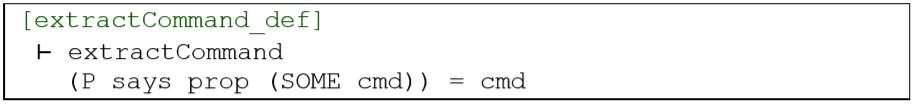
\includegraphics[width=0.6\linewidth]{extractCommand.PNG}
\end{figure}

 \item \underline{commandList}\\
  \textit{commandList} mapped \textit{extractCommand} onto an input list.  Thus, the result was a list of
  commands.  The definition for the \textit{commandList} was shown below.\\
  
  \begin{figure}[h]
  \centering
  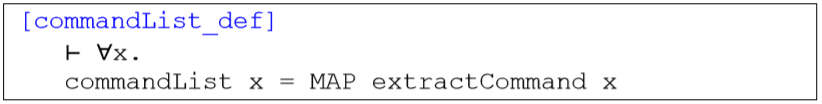
\includegraphics[width=0.6\linewidth]{commandList.PNG}
\end{figure}

 \item \underline{extractPropCommand}\\
  \textit{extractPropCommand} took an ACL request and extracted the proposition part of the request.
  The definition for it was shown below.\\
  \begin{figure}[h]
  \centering
  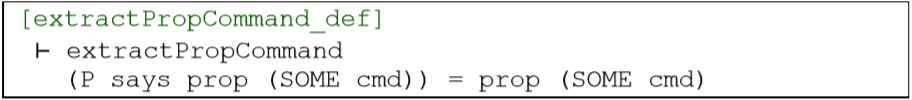
\includegraphics[width=0.6\linewidth]{extractPropCommand.PNG}
\end{figure}

\item \underline{propCommandList}\\
  \textit{propCommandList} mapped \textit{extractPropCommand} onto an input list.  Thus, the result was a list of
  propositions.  The definition for \textit{propCommandList} was shown below.\\
  \begin{figure}[h]
  \centering
  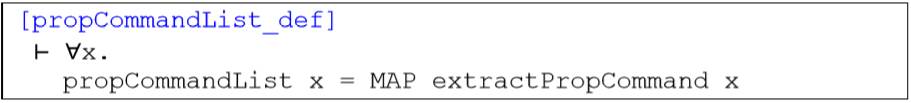
\includegraphics[width=0.6\linewidth]{propCommandList.PNG}
\end{figure}

 \item \underline{extractInput}\\
  \textit{extractInput} took an ACL formula and extracted the input x.   The definition for \textit{extractInput}
  was shown below.\\
  \begin{figure}[h]
  \centering
  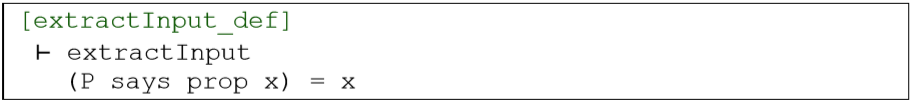
\includegraphics[width=0.6\linewidth]{extractInput.PNG}
\end{figure}

 \item \underline{inputList}\\
  \textit{inputList} mapped \textit{extractInput} onto an input list.  Thus, the result was a list of inputs.
  The definition for \textit{inputList} was shown below.\\
  \begin{figure}[h!]
  \centering
  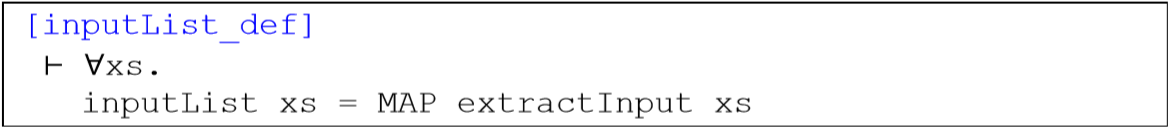
\includegraphics[width=0.6\linewidth]{inputList.PNG}
\end{figure}

 \item \underline{Theorems and Definitions}\\
  The remainder of the theorems and definitions were the same as in ssm11 except for changes that
  accomodated the different format of the input.  For the sake of brevity, the reader should view
  the EmitTeX pretty-printed files for ssm.
  
  \end{itemize}
 

\section{Secure State Machines Descriptions}
\label{sec:secure-state-mach}

\subsection{Top-level Secure State Machine}
\label{sec:top-level-secure}

\begin{figure}[h]
  \centering
  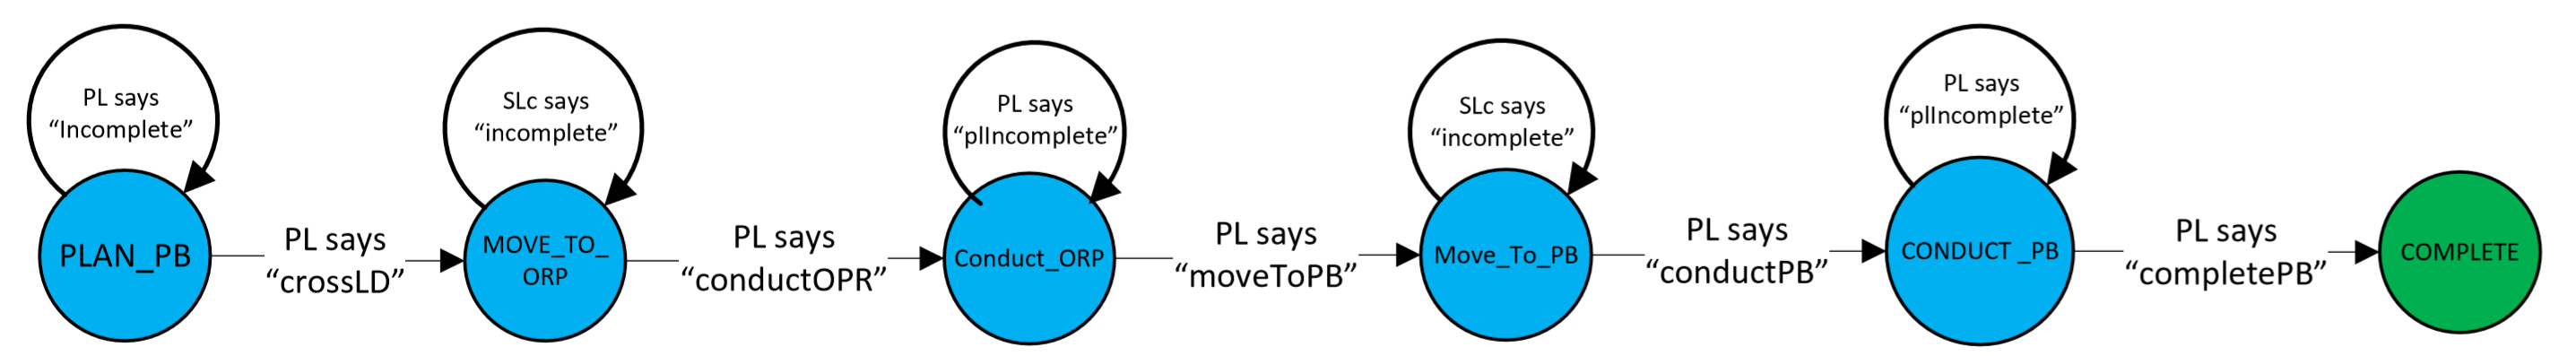
\includegraphics[width=1\linewidth]{diagram.PNG}
\end{figure}


rte






% ---- this points LaTeX to PatrolBaseDoc.tex ----
% Local Variables:
% TeX-master: "../PatrolBaseDoc"
% End: